\documentclass[twocolumn]{rbef}


\usepackage{lipsum}

\usepackage{bbm}
\usepackage{subfig}
\usepackage{pdfpages} % Para incluir a capa.

\newcommand{\1}{\mathbbm{1}}
\newcommand{\s}{\mathcal{S}}
\newcommand{\T}{\mathcal{T}}
\newcommand{\A}{\mathcal{A}}
\newcommand{\ket}{\rangle}
\newcommand{\bra}{\langle}

\newtheorem{defi}{Definição}
\newtheorem{theorem}{Teorema}
\newtheorem{acknowledgement}[theorem]{Acknowledgement}
\newtheorem{algorithm}[theorem]{Algorithm}
\newtheorem{axiom}[theorem]{Axiom}
\newtheorem{claim}[theorem]{Claim}
\newtheorem{conclusion}[theorem]{Conclusion}
\newtheorem{condition}[theorem]{Condition}
\newtheorem{conjecture}[theorem]{Conjecture}
\newtheorem{corollary}[theorem]{Corollary}
\newtheorem{criterion}[theorem]{Criterion}
\newtheorem{definition}[theorem]{Definition}
\newtheorem{example}[theorem]{Example}
\newtheorem{exercise}[theorem]{Exercise}
\newtheorem{lemma}[theorem]{Lemma}
\newtheorem{notation}[theorem]{Notation}
\newtheorem{problem}[theorem]{Problem}
\newtheorem{proposition}[theorem]{Proposition}
\newtheorem{remark}[theorem]{Remark}
\newtheorem{solution}[theorem]{Solution}
\newtheorem{summary}[theorem]{Summary}
\newenvironment{proof}[1][Proof]{\noindent\textbf{#1.} }{\ \rule{0.5em}{0.5em}}

\titulocabecalho{Utilizando a Regressão Logística para Classificação de Churn em um Ambiente de Startup}
\autorcabecalho{Antonio C. da Silva Júnior}

\numeracao{01}
\volume{01}
\numero{01}
\ano{2019}
\doi{http://dsbd.leg.ufpr.br/tcc}
% \tipodeartigo{TCC DSBD}
\tipodeartigo{Especialização em Data Science \& Big Data}
% \addtocounter{page}{566} %% \setcounter produces extra white page!!! use ===\addtocounter===

\author[1]{Antonio C. da Silva Júnior}

\affil[1]{Campus Santos, Universidade Paulista
  Av. Conselheiro Nébias 766, Boqueirão, 11045-002, Santos, SP,
  Brasil\thanks{\href{emailto:juniorssz@gmail.com}{juniorssz@gmail.com}}
}
% https://www.unip.br/presencial/universidade/campi/santos.aspx
% \author[2]{Alan C. Santos}

% \affil[2]{Instituto de Física, Universidade Federal Fluminense
%   Av. General Milton Tavares de Sousa s/n, Gragoatá, 24410-346, Niterói,
%   RJ, Brasil\thanks{\href{emailto:alancs@if.uff.br}{alancs@if.uff.br}}
% }

\titulo{Utilizando a Regressão Logística para Classificação de Churn em um Ambiente de Startup}

\subtitulo{Using Logistic Regression for Churn Classification in a Startup Environment}

% -----------------------------------------------------------------------

\begin{document}

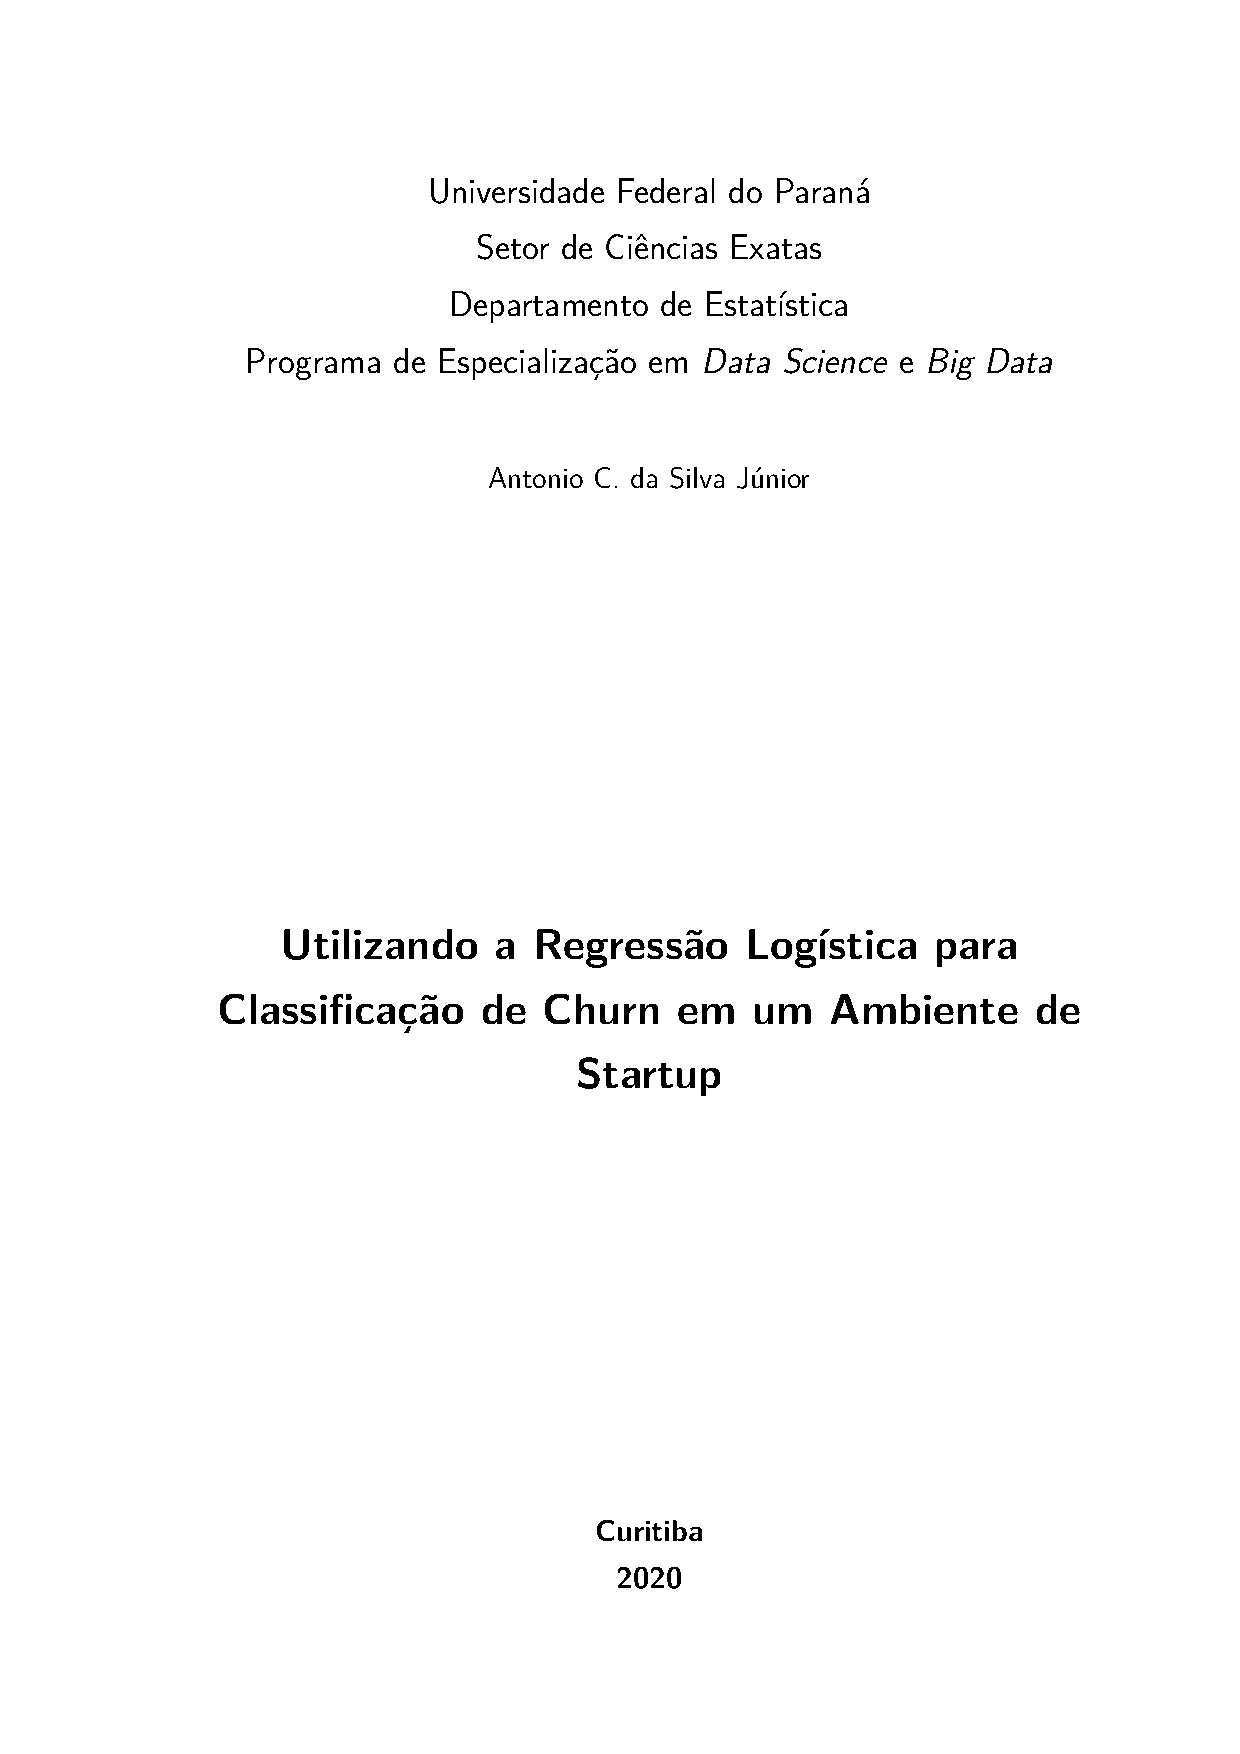
\includepdf[pages=-]{cover.pdf} % Incluí a capa

\begin{primeirapagina}

  % \begin{center}
  %   \vspace{-12pt} \small{Recebido em xxx. Aceito em xxx}
  % \end{center}

  \begin{abstract}
    Um desenvolvimento didático para determinar a solução da
    equação de movimento para uma partícula carregada imersa em
    uma região na presença de campos elétrico e magnéticos
    estáticos genéricos é proposto. Nossa proposta tem como
    alicerce a vantagem de, utilizando as propriedades da
    transformada de Laplace, podermos mapear um sistema de
    equações diferenciais não-homogêneas de segunda ordem no
    problema simples de encontrar as soluções de um sistema linear
    de equações. A partir da solução mais geral possível para o
    sistema, estudamos alguns casos particulares e recuperamos de
    forma simples alguns resultados já existentes na literatura. A
    fim de motivar nosso estudo, partimos do Teorema de Ehrenfest
    e discutimos como os resultados obtidos para o caso clássico
    podem ser interpretados na sua versão quântica.
    \palavraschave{movimento de cargas, campos elétrico e
      magnético, trajetória, análogo quântico}

  \end{abstract}

  \begin{otherlanguage}{english}


    \begin{abstract}
      A didactic development to determinate the solution of the
      motion equations for a charged particle under influence of
      electric and magnetic static fields is proposed. Our proposed
      uses the advantages and proprieties of the Laplace’s
      transformation, to map a system of N non-homogeneous
      differential equations of second order in a system composed by
      N linear equations. From the solution more general for
      dynamics of the system, we study some particular cases to
      recover, of a simple way, the results present in the
      literature. In order to give a motivation to our study, we use
      the Ehrenfest’s theorem and we discuss as the classical
      results can be interpreted in its quantum version.
      \keywords{Charge moving, electric and magnetic fields,
        trajectory, quantum analogue}

    \end{abstract}
  \end{otherlanguage}

\end{primeirapagina}
\saythanks

\hypertarget{introduuxe7uxe3o}{%
\section{Introdução}\label{introduuxe7uxe3o}}

A importância do relacionamento de longo prazo entre cliente e empresa é um assunto vastamente discutido na literatura. Segundo Ganesh, Arnold e Reynolds (2000), devido aos efeitos de aprendizado e à redução dos custos de manutenção, atender um cliente se torna menos dispendioso a cada ano adicional de relacionamento. Para Hennig-Thurau (2004), devido ao aumento dos custos para atração de novos clientes em um mercado competitivo e à potencial redução dos custos associados aos relacionamentos de longo prazo, a retenção de clientes se torna essencial para a sobrevivência e o sucesso econômico das empresas do setor de serviços. De acordo com Gallo (2014), dependendo do estudo e do segmento no qual a empresa está inserida, o custo para adquirir um novo cliente pode ser de cinco a vinte e cinco vezes superior ao da manutenção de um cliente já existente.

O desenvolvimento de estratégias para retenção de clientes se tornou uma prática comum entre empresas de diversos segmentos, e em consequência, antever o abandono de clientes passou a ser um anseio constante. Em um momento de concentração generalizada de esforços na direção da orientação a dados, os modelos preditivos para detecção de abandono de clientes, predominantemente utilizados por grandes companhias no setor de telecomunicações, se tornaram ferramentas populares nas empresas, independentemente da magnitude e da área de atuação.

A literatura comprova que a modelagem preditiva de abandono de clientes, também conhecida como modelagem preditiva de churn, é um tema bastante explorado e que possibilita inúmeras maneiras de desfecho: Botelho e Tostes (2010) ajustaram um modelo de regressão logística para predizer a probabilidade de churn em uma grande empresa de varejo; Vafeiadis et al.~(2015) tiveram sucesso, entre os métodos comparados, na classificação de churn através do SVM (kernel polinomial) com AdaBoost em uma empresa de telecomunicações; Com base nos dados de avaliações online de clientes, Kumar e Yadav (2020) propuseram um modelo preditivo de churn baseado em regras através de redes neurais artificiais e teoria dos conjuntos aproximados.

Com base nos dados de uma startup brasileira que tem como principal produto uma plataforma digital para conectar vendedores de diversos segmentos aos grandes marketplaces, a proposta deste artigo é apresentar um modelo preditivo que possibilite não só a classificação de vendedores propensos a abandonar a empresa, mas que também permita a interpretação dos motivos que possivelmente estejam impactando a predição. Diante da variedade de técnicas disponíveis e das particularidades de cada modelo de negócio, a escolha do algoritmo adequado se torna uma etapa crucial do processo de modelagem. Portanto, tendo como referência a abordagem de Silva Júnior, Almeida e Santos (2020), que utilizaram uma modelagem híbrida multicritério considerando múltiplos decisores para a escolha de um modelo preditivo de churn, o algoritmo escolhido para desenvolver o classificador proposto foi a regressão logística.

\hypertarget{materiais-e-muxe9todos}{%
\section{Materiais e métodos}\label{materiais-e-muxe9todos}}

\hypertarget{estruturauxe7uxe3o-do-conjunto-de-dados}{%
\subsection{Estruturação do conjunto de dados}\label{estruturauxe7uxe3o-do-conjunto-de-dados}}

Os dados utilizados neste trabalho referem-se a clientes de uma startup paranaense, anonimizados e com variáveis variáveis quantitativas padronizadas com média 0 e desvio padrão 1. Considerando que estes clientes contrataram uma plataforma digital que possibilita a venda de produtos nos principais marketplaces, neste trabalho eles serão chamados de vendedores. Devido às características da arquitetura do banco de dados e às particularidades do negócio da companhia, houve a necessidade de realizar um longo processo de data wrangling. De acordo com Kandel et al.~(2011), este processo inicia-se por um diagnóstico preliminar dos dados, ou seja, se estão no formato adequado, se respondem as perguntas que motivaram a análise e o que é necessário para colocá-los no formato ideal. Em seguida avalia-se a ocorrência de dados faltantes, valores inconsistentes e duplicatas e, por fim, realiza-se um processo de limpeza e transformação, de modo a se obter um conjunto de dados adequado para o estudo.

\hypertarget{definiuxe7uxe3o-da-resposta-e-covariuxe1veis-de-desempenho}{%
\subsubsection{Definição da resposta e covariáveis de desempenho}\label{definiuxe7uxe3o-da-resposta-e-covariuxe1veis-de-desempenho}}

Inicialmente foram definidos como churn = 1 os vendedores que estiveram inativos por 30 dias corridos desde a data da última atividade e permaneceram no mesmo estado definitivamente, considerando como atividade o acesso à plataforma digital ou a ocorrência de uma venda online. Em seguida, em função da data de corte estabelecida conforme a Tabela \ref{tab:dataDeCorte}, foram mantidos no conjunto de dados somente os vendedores com pelo menos 90 dias de histórico. O período de 90 dias, finalizado na data de corte, foi dividido igualmente em dois períodos, onde foram calculadas métricas como faturamento, ticket médio, quantidade de produtos publicados, quantidade de pedidos em cancelados, número de dias em atividade e etc., em cada um dos quadrantes. Em seguida, através da Equação \eqref{eq:desempenho}, foi calculado desempenho do vendedor em função de diversas métricas, onde \(V1\) e \(V2\) são os valores calculados em cada período.

As métricas desempenho, data à natureza da equação de origem, possuem o comportamento explicado pela Tabela \ref{tab:metricas}. Ao término desta etapa foi obtido um conjunto de dados composto pela variável resposta (churn) e, como covariáveis, 10 métricas de desempenho, onde cada observação representa um vendedor.

\begin{table}

\caption{\label{tab:dataDeCorte}Definição da data de corte}
\centering
\fontsize{8}{10}\selectfont
\begin{tabular}[t]{ll}
\toprule
Vendedor & Data de corte\\
\midrule
Definido como churn & Última atividade\\
Em atividade normal & Realização da análise\\
\bottomrule
\end{tabular}
\end{table}

\begin{equation}
Desempenho = \dfrac{V2}{V1+V2} \label{eq:desempenho}
\end{equation}

\begin{table}

\caption{\label{tab:metricas}Interpretação das métricas de desempenho}
\centering
\fontsize{8}{10}\selectfont
\begin{tabular}[t]{ll}
\toprule
Valor & Desempenho\\
\midrule
0,5 & Mantido\\
> 0,5 & Aumentado\\
< 0,5 & Reduzido\\
\bottomrule
\end{tabular}
\end{table}

\hypertarget{adiuxe7uxe3o-de-outras-covariuxe1veis}{%
\subsubsection{Adição de outras covariáveis}\label{adiuxe7uxe3o-de-outras-covariuxe1veis}}

Foram adicionadas covariáveis qualitativas que representam o estágio do vendedor, o plano contratado e a região de origem, bem como covariáveis quantitativas como o faturamento total, total de produtos publicados, quantidade total de pedidos e etc., resultando em um conjunto de dados com 26 covariáveis.

\hypertarget{criauxe7uxe3o-de-covariuxe1veis-binuxe1rias}{%
\subsubsection{Criação de covariáveis binárias}\label{criauxe7uxe3o-de-covariuxe1veis-binuxe1rias}}

De acordo com Fávero e Belfiore (2017), dada a necessidade de analisar o comportamento da variável resposta em função de uma covariável qualitativa com \(n\) categorias, deve-se criar \(n-1\) covariáveis binárias (dummies), que assumem valores iguais a 0 ou 1, ficando por conta do pesquisador decidir qual das categorias será a referência (dummy = 0). Portanto, as covariáveis qualitativas adicionadas foram transformadas em binárias, resultando em um conjunto de dados composto por 35 variáveis e 11.131 observações, representado através da Tabela \ref{tab:dicionario}.

\begin{table}

\caption{\label{tab:dicionario}Dicionário do conjunto de dados estruturado}
\centering
\fontsize{8}{10}\selectfont
\begin{table*}{lll}
\toprule
Variável & Tipo & Descrição\\
\midrule
y & binária & Churn\\
x1 & numérica & Desemp. - pedidos\\
x2 & numérica & Desemp. - dias em atividade\\
x3 & numérica & Desemp. - pedidos cancelados ou suspensos\\
x4 & numérica & Desemp. - envios com atraso\\
\addlinespace
x5 & numérica & Desemp. - envios com atraso (dias)\\
x6 & numérica & Desemp. - entregas com atraso (dias)\\
x7 & numérica & Desemp. - faturamento\\
x8 & numérica & Desemp. - produtos cadastrados\\
x9 & numérica & Desemp. - categorias cadastradas\\
\addlinespace
x10 & numérica & Desemp. - ticket médio\\
x11 & numérica & Desemp. - razão dos preços de frete e pedido\\
x12 & binária & Necessita de dias adicionais para postagem\\
x13 & binária & Estágio atual: B\\
x14 & binária & Estágio atual: I\\
\addlinespace
x15 & binária & Estágio atual: R\\
x16 & binária & Plano contratado: L\\
x17 & binária & Plano contratado: M\\
x18 & binária & Plano contratado: S\\
x19 & binária & Região de origem: Nordeste\\
\addlinespace
x20 & binária & Região de origem: Norte\\
x21 & binária & Região de origem: Sudeste\\
x22 & binária & Região de origem: Sul\\
x23 & numérica & Fluxo de caixa\\
x24 & numérica & Tamanho do portfólio\\
\addlinespace
x25 & numérica & Total de produtos cadastrados\\
x26 & numérica & Total de marcas cadastradas\\
x27 & numérica & Total de categorias cadastradas\\
x28 & numérica & Preço médio dos produtos publicados\\
x29 & numérica & Total de produtos publicados\\
\addlinespace
x30 & numérica & Total de pedidos\\
x31 & numérica & Total faturado\\
x32 & numérica & Dias desde a contratação até a primeira venda\\
x33 & numérica & Dias desde a contratação até o setup\\
x34 & numérica & Dias em atividade\\
\bottomrule
\end{table*}
\end{table}

\hypertarget{modelos-de-regressuxe3o-loguxedstica-binuxe1ria}{%
\subsection{Modelos de regressão logística binária}\label{modelos-de-regressuxe3o-loguxedstica-binuxe1ria}}

De acordo com Fávero e Belfiore (2017), o objetivo da regressão logística binária é o estudo da probabilidade de ocorrência de um evento de interesse (\(Y\)), apresentado na forma dicotômica (\(Y=1\) se o evento de interesse ocorrer; \(Y=0\), caso contrário), em função de um vetor vetor de covariáveis (\(X_1, ..., X_n\)). Sua definição ocorre através da Equação \eqref{eq:logito}, onde \(\beta_j\) (\(j = 0,1,2,...,p\)) representam os parâmetros a serem estimados, sendo \(\beta_0\) o intercepto e os demais, parâmetros de cada covariável, e o subscrito \(i\) representa cada observação da amostra (\(i = 1, 2,...,n\)).
\begin{equation}
ln \left ( \dfrac{\pi_i}{1-\pi_i} \right ) = \beta_0 + \beta_1 X_{i1} + ... +  \beta_p X_{ip}\label{eq:logito}
\end{equation}

A Equação \eqref{eq:logito}, conhecida como logito, modela a log-chance de ocorrência do evento de interesse. Portanto, para obter uma expressão para a probabilidade de ocorrência do evento, é necessário isolar matematicamente \(\pi_i\), resultando na Equação \eqref{eq:probabilidade}.
\begin{equation}
\pi_i = \dfrac{1}{1 + e^{-(\beta_0 + \beta_1 X_{i1} + ... +  \beta_p X_{ip})}}\label{eq:probabilidade}
\end{equation}

A estimação dos parâmetros \(\beta_i\) é realizada por máxima verossimilhança, método que consiste em encontrar, através da programação linear, os parâmetros que maximizam a função de verossimilhança representada através da Equação \eqref{eq:verossimilhanca}.
\begin{equation}
L =  \prod_{i=1}^{n} \left[ \pi^{Y_i} (1-\pi_i)^{1-Y_i} \right]\label{eq:verossimilhanca}
\end{equation}

Entretanto, matematicamente é mais conveniente trabalhar com o logaritmo da função de verossimilhança, conhecido como função de log-verossimilhança, representado através da Equação \eqref{eq:logverossimilhanca}, conforme destacam Fávero e Belfiore (2017) e Botelho e Tostes (2010).
\begin{equation}
logL = \sum_{i=1}^{n} \left\{ \left[Y_iln(\pi_i)\right] + \left[(1-Y_i)ln(1-\pi_i)\right] \right\}\label{eq:logverossimilhanca}
\end{equation}

\hypertarget{ajuste-e-anuxe1lise-dos-modelos-de-regressuxe3o-loguxedstica-binuxe1ria}{%
\subsubsection{Ajuste e análise dos modelos de regressão logística binária}\label{ajuste-e-anuxe1lise-dos-modelos-de-regressuxe3o-loguxedstica-binuxe1ria}}

\hypertarget{resultados}{%
\section{Resultados}\label{resultados}}

\hypertarget{conclusuxf5es}{%
\section{Conclusões}\label{conclusuxf5es}}

\hypertarget{referuxeancias}{%
\section*{Referências}\label{referuxeancias}}
\addcontentsline{toc}{section}{Referências}

\hypertarget{refs}{}
\leavevmode\hypertarget{ref-Botelho2010}{}%
BOTELHO, D.; TOSTES, F. D. Modelagem de probabilidade de churn. \textbf{Revista de Administração de Empresas}, v. 50, n. 4, p. 396--410, dez. 2010.

\leavevmode\hypertarget{ref-Favero2017}{}%
FÁVERO, L. P.; BELFIORE, P. \textbf{Manual de análise de dados: estatística e modelagem multivariada com Excel, SPSS e Stata}. {[}s.l.{]} Elsevier Brasil, 2017.

\leavevmode\hypertarget{ref-Gallo2014}{}%
GALLO, A. \textbf{The Value of Keeping the Right Customers}. Disponível em: \textless{}\url{https://hbr.org/2014/10/the-value-of-keeping-the-right-customers}\textgreater. Acesso em: 20 jul. 2020.

\leavevmode\hypertarget{ref-Ganesh2000}{}%
GANESH, J.; ARNOLD, M. J.; REYNOLDS, K. E. Understanding the Customer Base of Service Providers: An Examination of the Differences between Switchers and Stayers. \textbf{Journal of Marketing}, v. 64, n. 3, p. 65--87, jul. 2000.

\leavevmode\hypertarget{ref-HennigThurau2004}{}%
HENNIG-THURAU, T. Customer orientation of service employees. \textbf{International Journal of Service Industry Management}, v. 15, n. 5, p. 460--478, dez. 2004.

\leavevmode\hypertarget{ref-Kandel2011}{}%
KANDEL, S. et al. Research directions in data wrangling: Visualizations and transformations for usable and credible data. \textbf{Information Visualization}, v. 10, n. 4, p. 271--288, set. 2011.

\leavevmode\hypertarget{ref-Kumar2020}{}%
KUMAR, H.; YADAV, R. K. Rule-Based Customer Churn Prediction Model Using Artificial Neural Network Based and Rough Set Theory. In: \textbf{Advances in Intelligent Systems and Computing}. {[}s.l.{]} Springer Singapore, 2020. p. 97--108.

\leavevmode\hypertarget{ref-Junior2020}{}%
SILVA JÚNIOR, A. C. DA; ALMEIDA, I. D. P. DE; SANTOS, M. DOS. \textbf{Ordenação de algoritmos para modelagem preditiva de Churn: analisando o problema a partir dos métodos SAPEVO-M e VIKOR}. Congresso Internacional de Administração. \textbf{Anais}\ldots out. 2020

\leavevmode\hypertarget{ref-Vafeiadis2015}{}%
VAFEIADIS, T. et al. A comparison of machine learning techniques for customer churn prediction. \textbf{Simulation Modelling Practice and Theory}, v. 55, p. 1--9, jun. 2015.

\end{document}
